\clearpage
\section{Implementazione}

\subsection{Progettazione Architetturale}

\subsubsection{Requisiti non funzionali}
TODO\\
riassumere requisiti non funzionali progetto, spiegando vantaggi cloud\\
\subsubsection{Scelte tecnologiche}

TODO\\
cloud, azure\\
Firebase authentication, azure functions, azure pubsub\\
Flutter, C\#\\


\subsubsection{Scelta dell'architettura}
\begin{figure}[h!]
    \begin{center}
        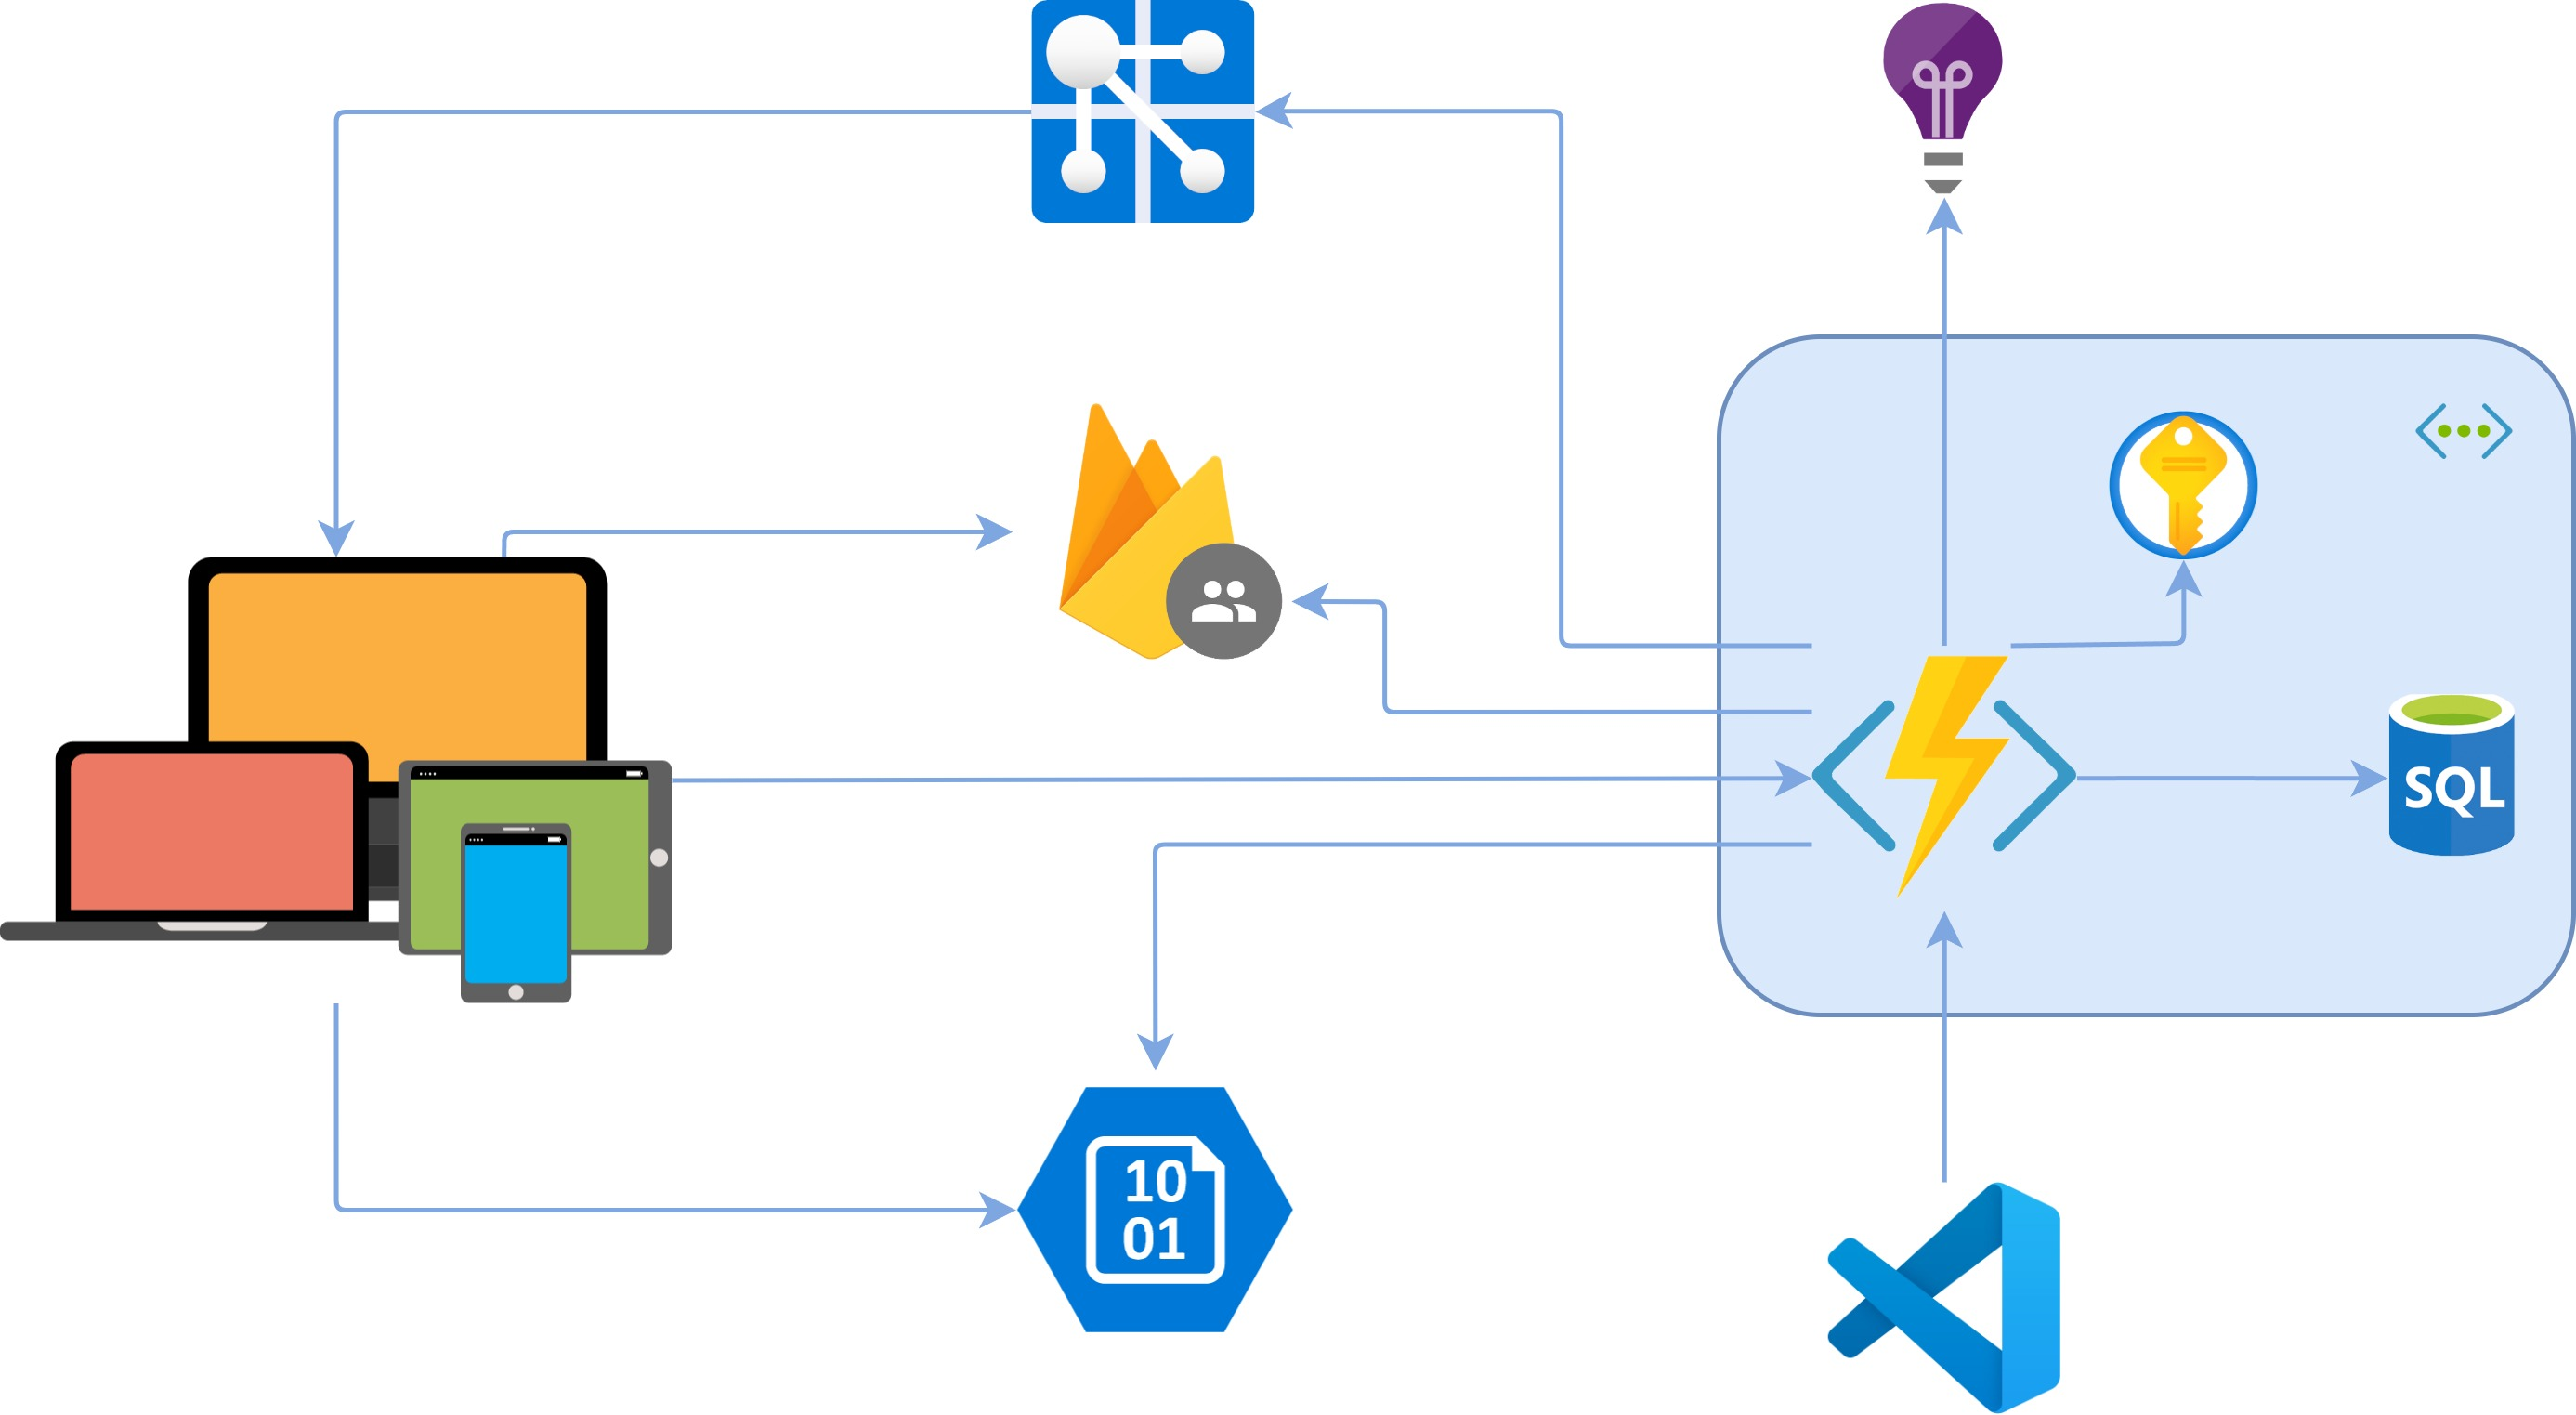
\includegraphics[width=\textwidth]{ImplementazioneArchitettura.jpg}
    \end{center}
\end{figure}
\subsection{Sicurezza}
TODO\\
Autentication tokens, canali sicuri(Https), scelte di limitazione dati e generazione hash.\\
ddos gestito dal cloud\\
log login gestito dal cloud\\
necessità sistema di monitoraggio log e integrazione sicurezza nello sviluppo, durante CI/CD\\

\newpage
\subsection{Progettazione di dettaglio}

Di seguito verranno riportate solo le modifiche principali rispetto al piano di progettazione
\subsubsection{Struttura}
TODO\\
Functions\\
divisione responsabilità tra componenti: controller, service e API\\
\subsubsection{Interazione}
TODO controlla condivisione con gruppi e salvataggio immagini
\newpage

\subsection{Deployment}

\subsubsection{Deployment Type-Level}

\begin{figure}[h!]
    \begin{center}
        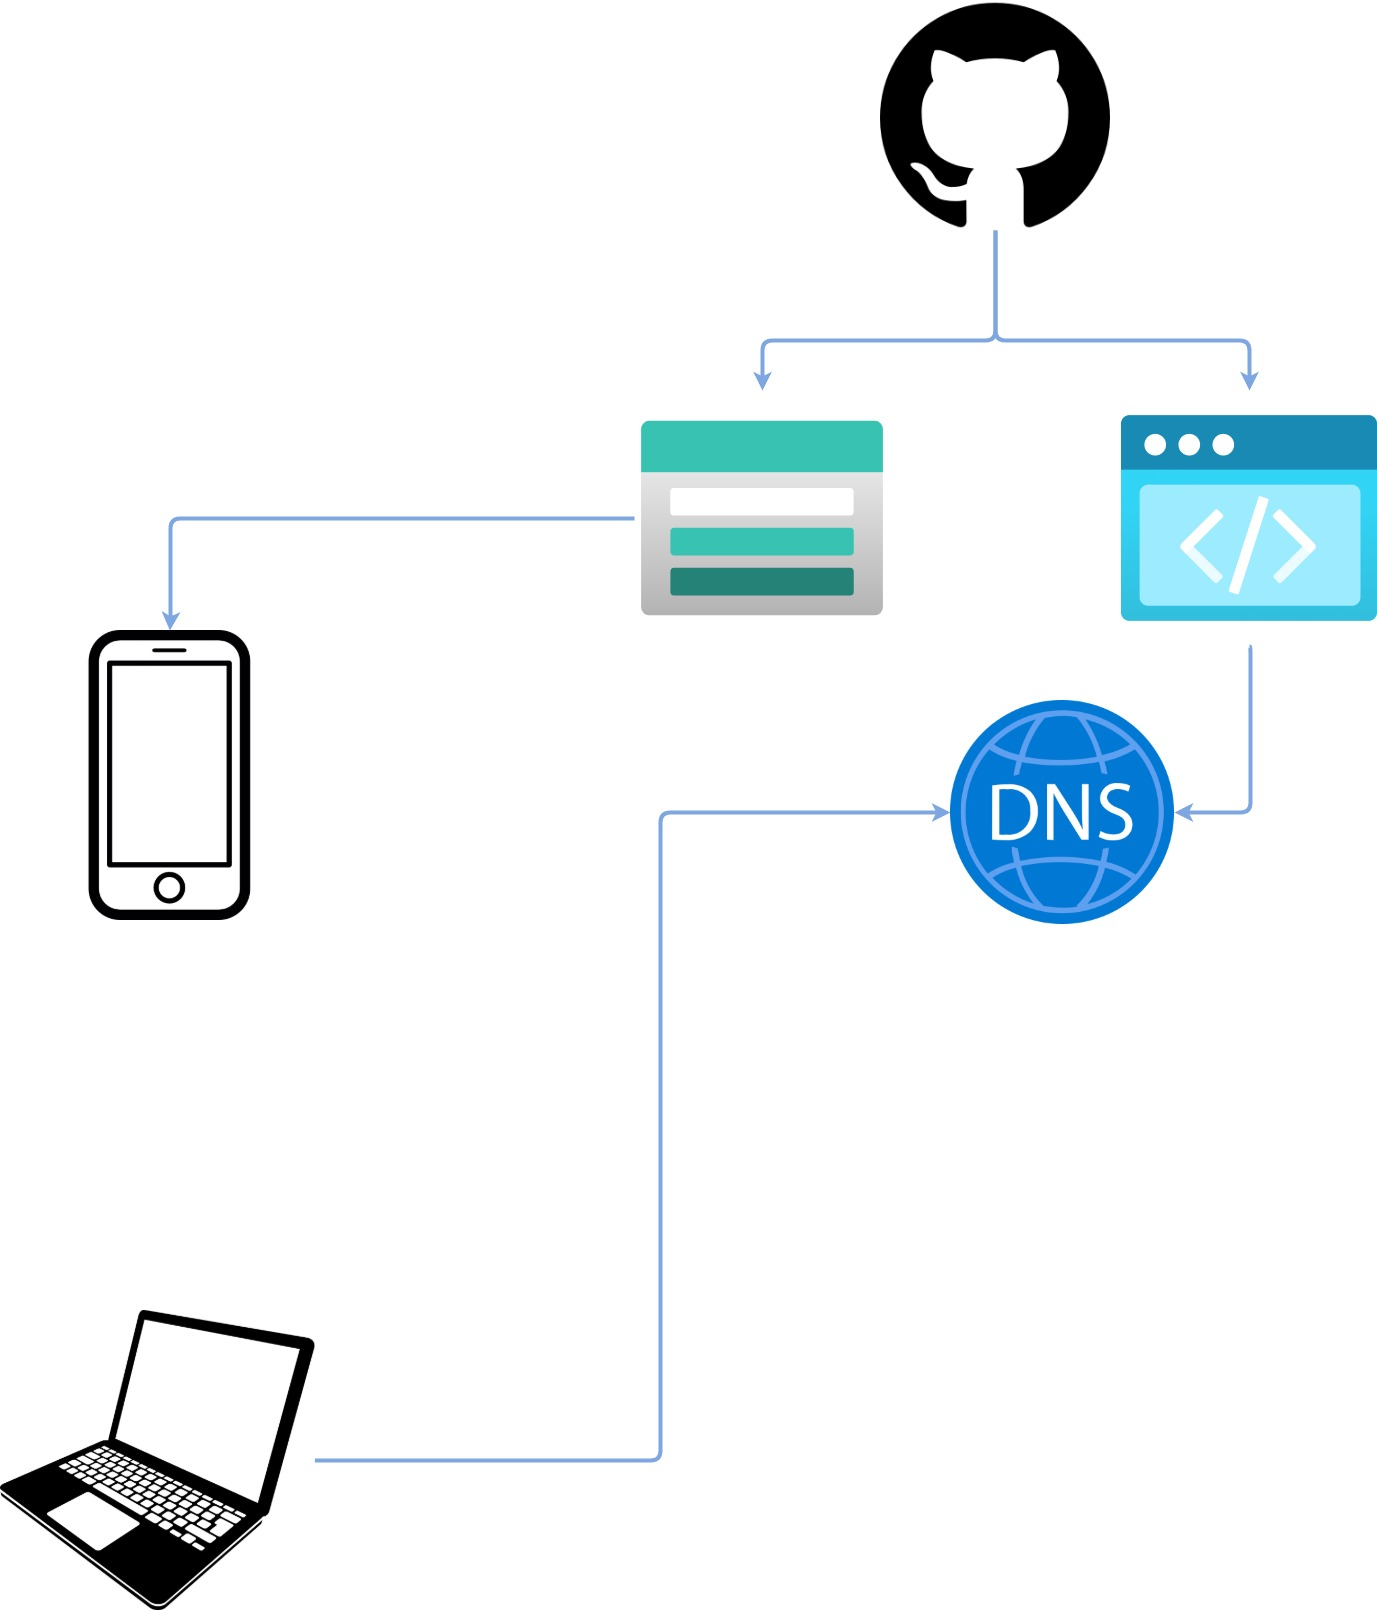
\includegraphics[width=\textwidth]{ImplementazioneDeployment.jpg}
    \end{center}
\end{figure}
Aggiornamento lato web gestito automaticamente, lato applicazione tramite notifica che chiederà all'utente di aggiornare la sua applicazione.
\newpage
\subsection{Testing e Performances}
